\documentclass[border=10pt]{standalone}
\usepackage{pgfplots}
\pgfplotsset{compat=1.18}
\begin{document}
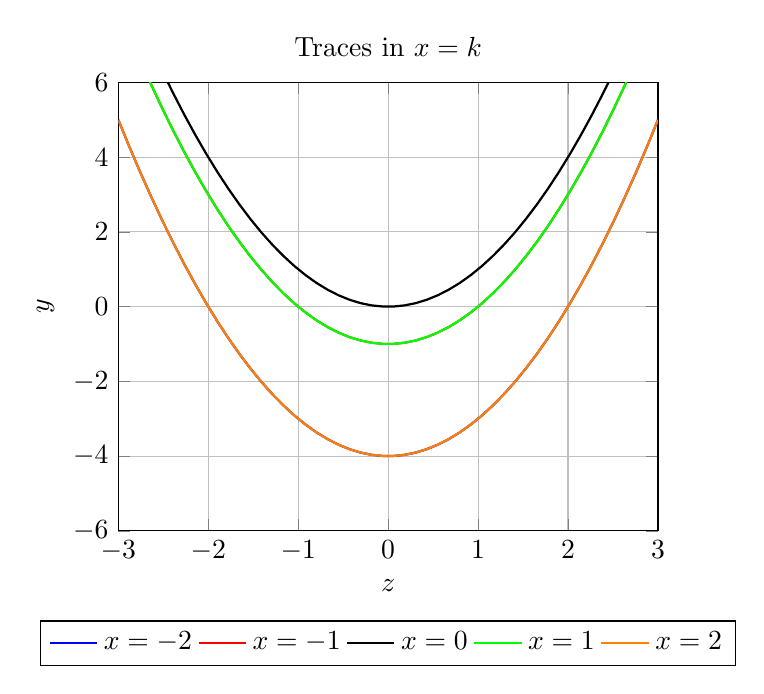
\begin{tikzpicture}
\begin{axis}[
    xlabel={$z$},
    ylabel={$y$},
    title={Traces in $x=k$},
    domain=-3:3,
    samples=50,
    grid=major,
    legend style={at={(0.5,-0.2)}, anchor=north, legend columns=-1},
    ymin=-6, ymax=6,
    xmin=-3, xmax=3
]
\addplot[blue, thick] {x^2 - 4}; \addlegendentry{$x=-2$}
\addplot[red, thick] {x^2 - 1}; \addlegendentry{$x=-1$}
\addplot[black, thick] {x^2}; \addlegendentry{$x=0$}
\addplot[green, thick] {x^2 - 1}; \addlegendentry{$x=1$}
\addplot[orange, thick] {x^2 - 4}; \addlegendentry{$x=2$}
\end{axis}
\end{tikzpicture}
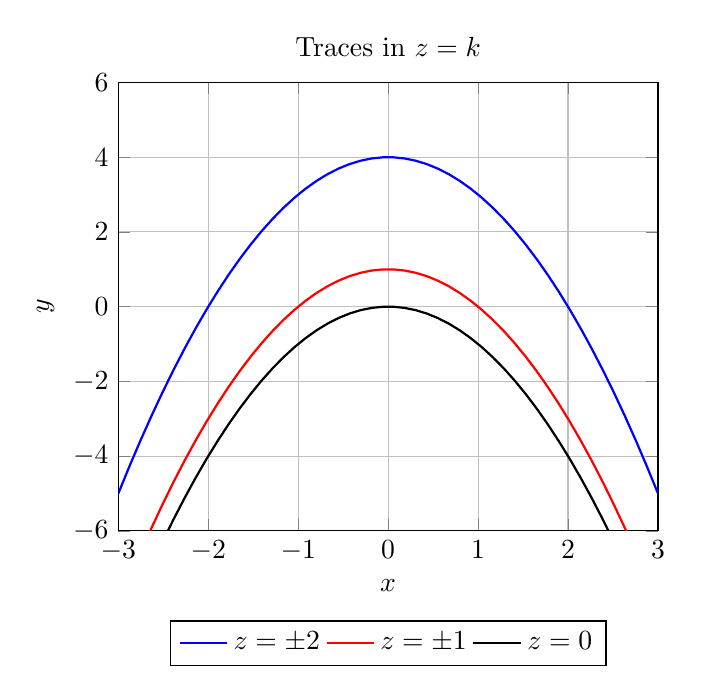
\begin{tikzpicture}
\begin{axis}[
    xlabel={$x$},
    ylabel={$y$},
    title={Traces in $z=k$},
    domain=-3:3,
    samples=50,
    grid=major,
    legend style={at={(0.5,-0.2)}, anchor=north, legend columns=-1},
    ymin=-6, ymax=6,
    xmin=-3, xmax=3
]
\addplot[blue, thick] {4 - x^2}; \addlegendentry{$z=\pm2$}
\addplot[red, thick] {1 - x^2}; \addlegendentry{$z=\pm1$}
\addplot[black, thick] {-x^2}; \addlegendentry{$z=0$}
\end{axis}
\end{tikzpicture}
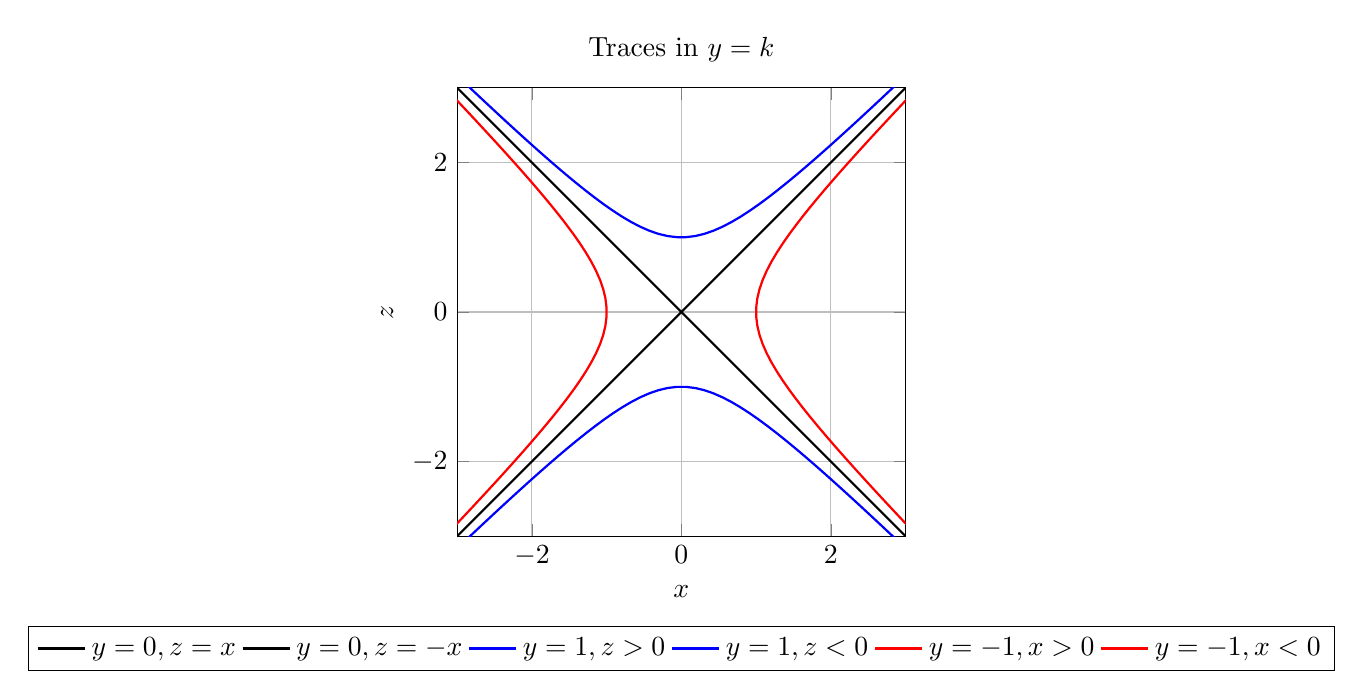
\begin{tikzpicture}
\begin{axis}[
    xlabel={$x$},
    ylabel={$z$},
    title={Traces in $y=k$},
    domain=-3:3,
    samples=50,
    grid=major,
    legend style={at={(0.5,-0.2)}, anchor=north, legend columns=-1},
    ymin=-3, ymax=3,
    xmin=-3, xmax=3,
    axis equal image
]
\addplot[black, thick] {x}; \addlegendentry{$y=0, z=x$}
\addplot[black, thick] {-x}; \addlegendentry{$y=0, z=-x$}
\addplot[blue, thick] {sqrt(x^2 + 1)}; \addlegendentry{$y=1, z>0$}
\addplot[blue, thick] {-sqrt(x^2 + 1)}; \addlegendentry{$y=1, z<0$}
\addplot[red, thick] (sqrt(x^2 + 1), x); \addlegendentry{$y=-1, x>0$}
\addplot[red, thick] (-sqrt(x^2 + 1), x); \addlegendentry{$y=-1, x<0$}
\end{axis}
\end{tikzpicture}
\end{document}